
\chapter{Background}

\label{ch:background}

\section{Introduction}

Interactive table is by no means a new idea. A lot of research has
been undertaken to find a simple suitable solution for the problem.

\subsection{Huddle Lamp}

The research into HuddleLamp\cite{huddle-link}, is the work that
is most similar to mine. HuddleTable is an extension from HuddleLamp.
HuddleLamp is a project trying to rectify  the fact that interactive
tables are quite expensive; making it is inaccessible for some everyday
consumers such as schools, public libraries, community centers etc.
HuddleLamp aim to use the multitude of unused tablets and smart-phones,
which people have lying around and create an ad-hoc interactive table
by using a novel sensing and detection method to deduce where the
devices are and what they should be shown.

HuddleLamp\cite{huddelamp-paper} proposes to use some of the cheaper
off-the-shelf products like a webcam, and a lamp to create a cheaper
interactive table that anyone could use. HuddleLamp proposes to use
a hybrid sensing approach that uses RGB and depth data, that can be
obtained from sophisticated webcams, which can detect and identify
mobile displays on tables and track their positions and orientations
. The project devised a way that multiple devices can interact with
each other in such a way that they all serve as one seamless multi-device
user interface.

Some of the main advantages of HuddleLamp were the face that you seam-less,
ad-hoc way of adding devices to the user interface (UI). Using HuddleLamp,
users can add or remove displays and reconfigure them in space without
the need of installing any software or attaching markers. Placing
them below the camera implicitly does the setup and pairing of devices.
Opening a URL on the device and making it visible to the camera adds
the new device to the \textquotedblleft Huddle\textquotedblright .
The camera also tracks the hand movements of the user, enabling interactions
between the devices.

The simplicity in adding a device to the table means users are not
constrained by having specific devices or requiring them to download
particular apps. This also means collaboration can occur on tables
that are cluttered with other objects likes pens and pencils. There
are 2 main components that are required for HuddleLamp;
a camera, they suggest Creative Senz3D camera, and a desk lamp, both
are relatively inexpensive components compared to an interactive table.

However there are some deficiencies in this improvisation to make
an interactive table. At the time of writing, the project has not
released a public version of their software. The developer
version requires you to connect a computer with the webcam, which
does most of the grunt work in term tracking devices. In this architecture
of HuddleLamp, this does all the resource intensive tasks so if it is
not a really powerful computer, users could experience lag. The fact
that to set this interactive table up you need to connect a lamp up
to a computer means that the whole setup is not very portable. The
size of the interactive part of the table is constrained by how high
up the camera is, from the surface of the table. The use of camera
means users arms and hands can sometimes impede the
detection and tracking of devices during moving or touching the devices.
Also the suggested camera and its software development kit (SDK) required
for the project has been taken off the market by its producer. Making
it imperative that an alternative to HuddleLamp is identified.


\subsection{ConnecTable}

\begin{figure}[H]
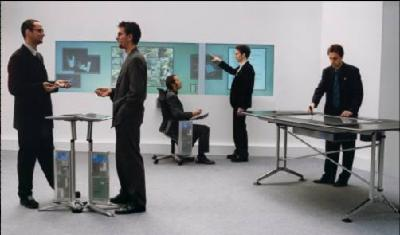
\includegraphics[scale=0.5]{connectables}

\protect\caption{ConnecTable Configuration}
\end{figure}


ConnecTable\cite{connectables} was one of the first attempt at creating
an interactive table. It is a mobile, context aware
information appliance, which uses a pen-based interaction. It uses
a dynamic, flexible coupling of displays to circumvent the limitation
of display real estate. By using in built sensors it has the ability
to merge displays when they come together to form a homogeneous physical
display. When 2 or more ConnecTables are connected, users are able
to exchange information by shuffling them over to the other display.
It predominantly has a pen based interaction, however it also sensors
integrated onto the tabletop to translate physical actions in the
real world to interactions on the tables. 

ConnecTable uses the movement in real space and engagement in discussions
between users as cues on when to connect with other tables. It also
has multiple use modes where two tables could connect together to
become a homogeneous display, or it could connect together to have
two simultaneous displays. Where both users can see and interact on
the same object in different screens, similar to group collaboration
in a Google Doc. ConnecTable uses transponders based on radio frequency
technology and electromagnetic ways for its sensing technology. The
table has a coil which emits an electromagnetic wave and a transponder
from the connecting table sends back its 32 bit identification number
back to the initiating table. The identification mechanism works in
range of around 3cm and takes nearly 1.5 seconds to complete.

\begin{figure}[h]

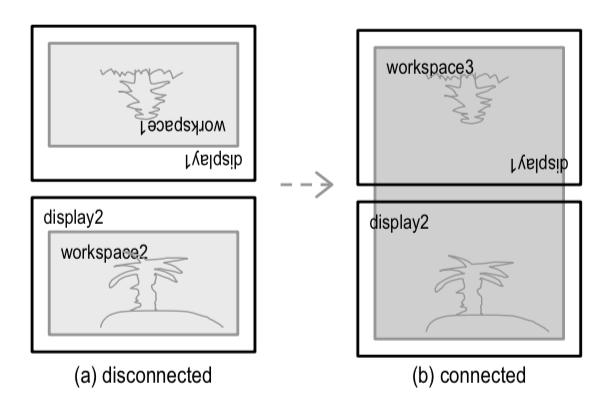
\includegraphics[scale=0.5]{connecTable_views}
\protect\caption{Shows the difference in views between connected and disconnected ConnecTables}
\end{figure}

\subsection{Beamatron}

\begin{figure}[H]
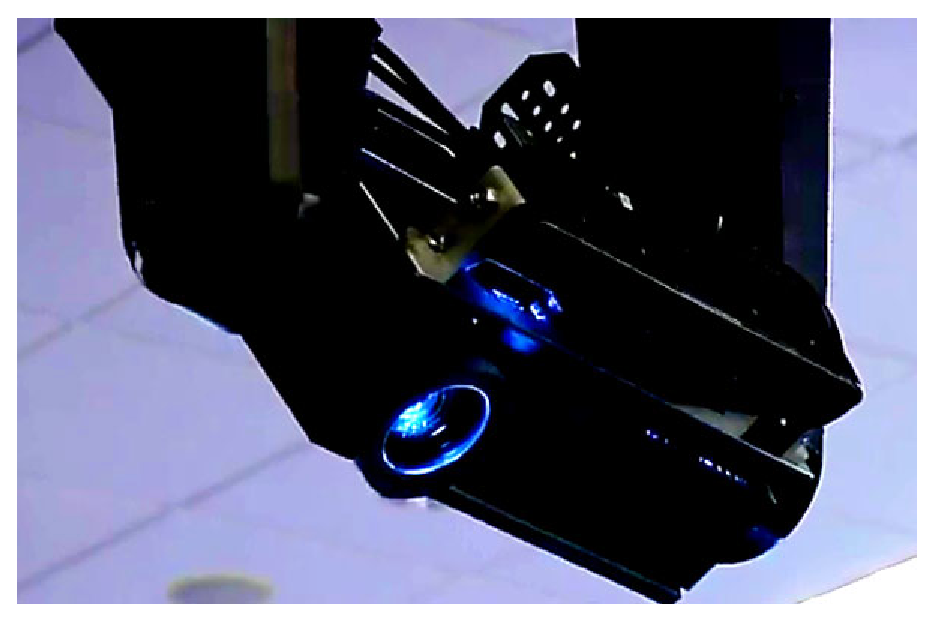
\includegraphics[scale=0.3]{Microsoft_Kinect_AR_Beamatron}

\protect\caption{Beamatron}


\end{figure}


Beamatron \cite{beamatron} is a contribution by the Microsoft research,
in to the fields of Spatial Augmented Reality. It uses depth cameras
with proprietary algorithms and techniques to render graphics precisely
onto the real world according the users point of view. By using a
depth camera they were able to add more modes of interaction to augmented
reality, i.e moving objects or holding onto object. It has the capabilities
to allow live changes on the projections. It can reason with room
coordinates and render 3D objects in precise orientation. Uses 3D
sound source localization as a means to track user position when the
user is not in view. 
Beamatron hardware consist of a video projector and a Microsoft Xbox
Kinect sensor mounted to a City Theatrical Autoyoke\cite{autoyoke}
moving light platform. To get the information about the pan and tilt
of the Autoyoke they had to create a bespoke circuit board which connected
to the respective encoders to Autoyoke giving Beamatron an accurate
hardware-based feedback which allows them to stabilise their graphics. 

One of the biggest shortcomings of placing a steerable display in
the center of the room is that the information received is limited
to the view of the single camera. They compensated for the lack of
depth information by mounting multiple 3 Kinect sensors to the corners
of the room and using triangulation to find sources of sound and in
turn identifying the presence of the user. They report some shortcomings
in their technique, especially when the user is standing beneath the
Beamatron usually fail.
The ideas and technique explored for Beamatron was intriguing. Especially
the positioning technique they used to locate the user when not in
the view of the depth camera. However the use of multiple Kinect sensors
and project fixed to the center of the view meant that the apparatus
was not portable. There was also quite an intense calibration method
required.


\subsection{LightSpace}
LightSpace
\begin{figure}[H]
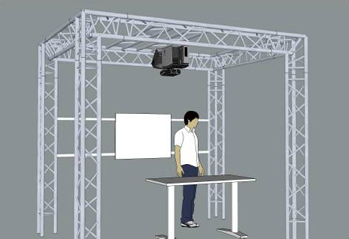
\includegraphics{LightSpace_configuration}

\protect\caption{LightSpace Configuration}
\end{figure}


\todo[inline]{background: finish lighstpace}


\subsection{SufacePhone}

SurfacePhone\cite{surfacephone} is a research concept which used
a projector in conjunction with a mobile device to project onto a
physical surface to allow tabletop like interaction in a mobile setup.
It has touch and gesture interaction incorporated into it giving a
realistic user experience. As the computing power of the mobile devices
increased and rivals a desktop, users wants to do increasingly complex
tasks on their mobile devices. However one of the main limitation
of mobile devices are their display size. 

SurfacePhone comes with a multitude of configurations. It could be
used as Single-device, Single User (SDSU) or the projections can merge
when multiple devices comes into proximity to make a Multi-device,
multi user interaction (MDMU) which creates a larger shared surface. 

Some of the troubles they came across with the devices was the actual
hardware. Since it required both a mobile device and projector, it
was a rather expensive tool to carry around with. Adding the projector
onto the phone meant the device was \uline{CHUNKY}. There was also
trouble with getting some aspects of interactions to work such as
Multi-modal touch.
\begin{figure}[H]
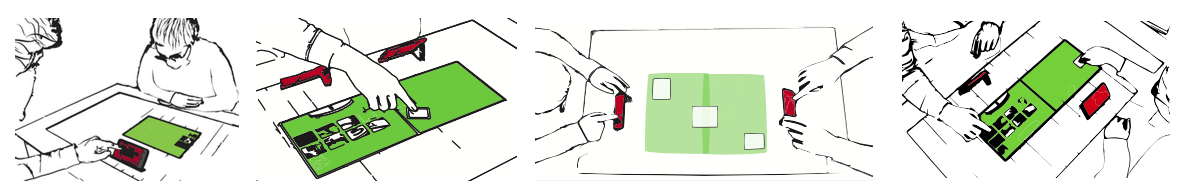
\includegraphics[scale=0.25]{surfacePhone}

\protect\caption{SurfacePhone}


\end{figure}

